\documentclass[11pt]{report}
\usepackage[utf8]{inputenc}
\usepackage{graphicx}
\usepackage{float}
\usepackage{subfig}
\usepackage[margin=0.5in]{geometry}
%\usepackage{caption}
%\usepackage{subcaption}
\usepackage{titlesec}
\usepackage{url}
\usepackage{amsmath,amsthm,enumitem,amsfonts}
\usepackage{mathtools}

\newtheorem{theorem}{Theorem}[section]
\newtheorem{lemma}[theorem]{Lemma}

\makeatletter
\newcommand*{\compress}{\@minipagetrue}
\makeatother

\DeclarePairedDelimiter\ceil{\lceil}{\rceil}
\DeclarePairedDelimiter\floor{\lfloor}{\rfloor}

%\usepackage{biblatex}

\titleformat{\chapter}{\Large\bfseries}{}{0pt}{\huge}
\titlespacing*{\chapter}{0pt}{0pt}{5pt}
\titleformat{\section}{\normalfont\bfseries}{}{0pt}{\large}
\titlespacing{\section}{0pt}{12pt plus 4pt minus 2pt}{5pt plus 2pt minus 2pt}
%\titlespacing{\subsection}{0pt}{12pt plus 4pt minus 2pt}{0pt plus 2pt minus 2pt}

\title{Report on\\Data Structures for Range Minimum Queries in Multidimensional Arrays}
\author{Chitradeep Dutta Roy, Zinnia Mukherjee}
\date{15 December, 2014}

\begin{document}

\maketitle

%\chapter{}
\section{Problem Definition}
This paper\cite{p10} addresses the problem of answering the range minimum query for higher dimensional arrays. Formally the range minimum query problem can be defined as follows:\par
For a d-dimensional array A of size $N = n_1.n_2...n_k$, where $n_k$ is the length of the $k^{th}$ dimension, a d-dimensional range minimum query problem aks for the minimum element in the query range $q = [a_1, b_1]$ x $[a_2, b_2]$ x..x $[a_d, b_d]$, where $a_k$ and $b_k$ are the upper and lower indices of the $k^{th}$ dimension respectively.
\begin{center}
\begin{math}
RMQ(A, q) = min A[q] = min_{(i_1,....,i_d)\in q}  A(i_1,....,i_d)
\end{math}
\end{center}
\section{Result and its importance}
This paper gives the first linear time and space preprocessing algorithm with constant query time for d-dimensional arrays where d is assumed to be fixed. In order to achieve this goal, new data structure has been proposed for which the following two conditions must be met:\par
\begin{enumerate}
\item It does not compute all the possible RMQ results at the preprocessing stage. Instead it allows the flexibility of comparisons and generating new results at the querying stage. This greatly reduces the number of types to linear.\par
\item The encoding of the data structure can be computed in linear time.
\end{enumerate}
Their result can be stated as follows:\par
For a d-dimensional array, $O((2.89)^d.(d+1)!)N)$ comparisons are sufficient to preprocess the input array and the querying stage requires O($2^d-1$) comparisons. Hence this gives a linear time preprocessing and constant time querying for higher dimensional arrays where d is assumed to be fixed. When this scheme is implemented under the RAM model with a fixed dimension, the querying time is increased to $O(3^d)$, which is still a constant, while the preprocessing time remains the same.\par
The RMQ problem for higher dimensional problems have been studied before and this paper made a major breakthrough by extending the 1D RMQ problem to higher dimensional arrays while preserving the linear time preprocessing and constant time querying features. The intial thought was to compute cartesian tree like structures in linear time which can also capture all possible RMQ results.\par
In fact, it was proved by Demaine, Landau and Weimann\cite{p2} that there is no such possible cartesian tree like structure in 2D case.
The results are fascinating since this builds upon the concept provided by Demaine et al. Their new idea of allowing constant time comparison at the querying stage changed the requirement of cartesian tree like structures. The main point of difference of their data structure with a cartesian tree is that while the latter requires to get range minimum without any comparison at the querying stage, their data structure allows a constant number of candidates to be compared at the querying stage. Many new research papers\cite{p14,p11,p12} have implemented this novel technique to come up with better query results in their specific domain.
\section{Impact of the results}
The range minimum query problem has direct impact in several fields related to string pattern matching, text compression, genomic sequence analysis in computational biology and image  processing. It also has applications in OLAP databases where multidimensional range min/max queries are used extensively.\par
Recently Brodal et al.\cite{p11} proposed a space efficient indexing data structure for two-dimensional RMQ problems that improves upon the $O(NlogN)$ bits or $O(N)$ words data structure proposed in this paper. Their paper uses the concept of Fibonacci lattice that has applications in the field of graphics and image processing. The paper by Mitzi et al.\cite{p12} explores the problem of expensive updating of prefix sum cubes for OLAP range queries on flash memory. This is based upon the theoretical research work being done on developing efficient data structures and algorithms that focus on range query computations for a given set of dimensions. Farzan et al. \cite{p14} presented a fully compressed representation of a set of m points on an $n$x$n$ grid that uses encoding in higher dimensions. This is again inspired by Yuan's contribution.


\newpage
%\chapter{}
\section{Previous Approaches}
Previously most of the data structures for solving 1D-RMQ problem were based on the following structure that there exists and $O(N)$-bit structure (built with no more than $N$ comparisons), i.e. the cartesian tree \cite{p9}, such that a query can be answered in $O(1)$ without any comparison with input elements. But is has been shown by Demaine, Landau and Weimann \cite{p2}, it is impossible to generalize the Cartesian tree to higher dimensions.

Gabow, Bentley and Tarjan \cite{p5}, first studied the RMQ problem in higher dimensions. They came up with an algorithm that uses dimensionality reduction to process a query recursively. The preprocessing complexity in their approach was $O(N\log^{d-1}N)$ time and space, and query can be answered in $O(\log^{d-1}N)$ time.

In multi-dimensional array setting, Chazelle and Rosenberg \cite{p3} gave an algorithm for range sum in semi-group model $(S, +)$ using $M$ units of storage where dimension $d$ is fixed and \( d \leq \log_{14} M/N\). Their preprocessing time complexity is $O(M)$ and query can be answered in \(O(\alpha^{d}(M,N))\) where $\alpha$ is functional inverse of Ackermann's function \cite{p8}.

Poon \cite{p6} gave a data structure for range max/min queries for $d$-dimensional OLAP datacubes, that can be build in $O((3n\log^*n)^d)$ time using $O((3n)^d)$ words. It can answer queries in $O(8^d)$ time.

Amir et al. \cite{p7} gave an algorithm for $2$D RMQ where they precompute the solution for a small number of micro blocks, where the size of each micro block is $O(s^2)$ with $s = \log^{[k]} n \text{ and } n = \sqrt N$. Their algorithm uses $O(kN)$ space, preprocessing time $O(N\log^{[k+1]}N)$ where $k > 1$ and query time is $O(1)$.
\section{New Approach}
We would describe the new approach \cite{p10} in 1-D case for the sake of brevity. It will be explained in multi-dimension setting in full report. The core idea behind this algorithm is a structure with the following properties,
\compress
\begin{itemize} \topsep0pt \itemsep1pt \parskip0pt \parsep0pt
  \item It does not need to completely capture the positions of all RMQ results, instead, it should be able to generate a constant number of candidates at the querying stage to compare.
  \item It can be computed in linear time.
\end{itemize}
Like conventional range trees \cite{p1}, the input array \(A\) is divided into canonical intervals which can be subdivided recursively into two halves until the size of an interval becomes $0$. There are $2^{k}$ such intervals for size $n/2^{k}$ where \(0 \leq k \leq \log n\), therefore total no of intervals is $2n-1$. For each canonical interval \( I = [a, b] \) the two following entries are computed, for \( a \leq x \leq b \),
\compress
\begin{itemize} \topsep0pt \itemsep1pt \parskip0pt \parsep0pt
  \item LeftMin\((I, x) = \min_{a \leq i \leq x \text{ and } i \in I} A[i] \)
  \item RightMin\((I, x) = \min_{x \leq i \leq b \text{ and } i \in I} A[i] \)
\end{itemize}
So there are total $O(n\log n)$ entries to be computed. Now for some $ I = [a,b] = I_1 \cup I_2 $ where $ I_1 = [a,b] \text{ and } I_2 = [b+1, c] $ the following algorithm can compute the above two values,
\compress
\begin{itemize} \topsep0pt \itemsep1pt \parskip0pt \parsep0pt
\item \( \text{LeftMin}(I, x) = \text{LeftMin}(I_1, x) \text{ if } x \in I_1 \)
\item \( \text{LeftMin}(I, x) = \text{LeftMin}(I_1, b) + \text{LeftMin}(I_2, x) \text{ if } x \in I_2 \)
\end{itemize}
Now \( \text{LeftMin}(I_2, x) \) can be computed in $O(\log(c-b+1))\) time using binary search of \( \text{LeftMin}(I_1, b) \) in precomputed LeftMin structure of $I_2$. Similarly RightMin structure can also be computed. The number of comparisons in the above Merge\((I_1,I_2)\) step is bounded by \(2\lceil {\log(l/2+1)} \rceil \leq 2\log_2l\). So the total complexity of the pre-processing step is given by the recurrence \(H(n) = 2H(n/2) + 2\log n \), solving the recurrence we get \( H(n) \leq 4n \).

Now a query RMQ\((A, q)\) where $q=[a,b]$ can be answered in $O(\log n)$ time by calling SolveQuery\(([1,n], q)\). Let's assume $I=[u,v]$, then following are the three cases
\compress
\begin{itemize} \topsep0pt \itemsep0pt \parskip0pt \parsep0pt
  \item If $a=u$ then answer is LeftMin\((I, b)\) or if $b=v$ it is RightMin\((I, a)\)
  \item If $I=I_1 \cup I_2$, and $q \subseteq I_1$ recursively call SolveQuery\((I_1, q)\) if $q \subseteq I_2$ call SolveQuery\((I_2, q)\)
  \item If $q$ overlap with both $I_1$ and $I_2$ then answer is $\min{\{\text{RightMin}(I_1,a),\text{LeftMin}(I_2, b)\}}$
\end{itemize}
We can reduce query processing time to $O(1)$, by building an auxiliary tree $T$ where node $v_I$ denotes interval $I=I_1 \cup I_2$ and its children would be $v_{I_1}$ and $v_{I_2}$. Then a nearest common ancestor data structure can be built using any of the techniques presented in \cite{p4}, \cite{p13}, \cite{p16}, \cite{p15}. And now for any query \(q=[a,b]\) the nearest common ancestor of two canonical intervals \( [a,a] \text{ and } [b,b] \) in $T$ in constant time. And it is can surely be answered by either by first or last case of the above in constant time.

For $d$-dimensional array it can be shown that the preprocessing requires $O((2.89)^d*(d+1)!)N$ comparisons and query can answered in $2^d-1$ using $d$ nearest common ancestor queries.


%\newpage
\section{1D RMQ: Preprocessing}
Let us consider an input array $A$ of size $[1 \ldots n]$. The preprocessing stage 
recursively divides the array $A$ into two sets of canonical intervals until the interval size becomes one. In this way we will get $2^i$ canonical intervals at the $i^{th}$ division stage and a total of $2n-1$ intervals.
For each canonical interval $I$, the following data structures are constructed:
\begin{center}
$LeftMin(I,x)=\min_{i \leq x \text{ and } i \in I}A[i]$ \\
$RightMin(I,x)=\min_{i \geq x \text{ and } i \in I}A[i]$
\end{center}
Computing the \emph{LeftMin} and \emph{RightMin} structures for intervals of length 1 is trivial. Now let $I_1=[a,b]$ and $I_2=[b+1,c]$ be the two neighbouring canonical intervals. The \emph{LeftMin} structure for $I=I_1 \cup I_2$ is merged from the \emph{LeftMin} structures of $I_1$ and $I_2$  as follows:
\begin{enumerate}
\item If $x \in I_1$, then $LeftMin(I, x)=LeftMin(I_1, x)$. This takes constant time.
\item If $x \in I_2$ and $s=LeftMin(I_1, b)$, then a binary search of $s$ is done in \emph{LeftMin} structure of $I_2$. As the \emph{LeftMin} entries are non-increasing, $LeftMin(I, x) = s,\ \forall LeftMin(I_2, x) \geq s$ and $LeftMin(I, x) = LeftMin(I_2, x),\ \forall LeftMin(I_2, x) < s$. Hence this step takes $\left \lceil{\log_{2}(|I_2|+1)}\right \rceil$ comparisons.
\end{enumerate}
We can compute \emph{RightMin} structures in a similar way. In order to merge the \emph{LeftMin} and  \emph{RightMin} structures of an interval of size $l$ from the \emph{LeftMin} and  \emph{RightMin} structures its two sub intervals of size $\frac{l}{2}$, the number of comaprisons is bounded by $2 \log_{2}l$. Let $H(n)$ denote the number of comparisons used to preprocess an array of size $n$, then we have $H(1)=0$ and for $n \geq 2$ we have, $H(n)=2H(\frac{n}{2})+ 2 \log n$. Hence from the logarithmic comparison merging process, we have $H(n) \leq 4n$.
\section{1D RMQ: Querying}
\textbf{Na\"{\i}ve Approach:} Suppose there is a query $q=[a, b]$ on interval $I=[u, v]$ and let $SolveQuery([u, v], q)$ denote the basic procedure which returns the range minimum value in $I$. Three cases will arise:
\begin{enumerate}
\item Case 1: If $a=u$, $LeftMin(I, b)$ is returned; else if $b=v$, $RightMin(I, a)$ is returned.
\item Case 2: If $I_1$ and $I_2$ are two canonical intervals split from $I$ and $q \subset I_1$, then recursively invoke \emph{SolveQuery($I_1$, q)}; else if $q \subset I_2$, then recursively invoke \emph{SolveQuery($I_2$, q)}.
\item Case 3: If $q$ overlaps between $I_1$ and $I_2$, then $q$ contains right boundary of $I_1$ and left boundary of $I_2$, hence range minimum value is $= \min \{ RightMin(I_1, a), LeftMin(I_2, b) \}$.
\end{enumerate}
Although Case 1 and Case 3 takes $0$ and $1$ comparisons respectively, Case 2 is an $\mathcal{O}( \log n)$ operation where $n$ is the size of the initial input array. To bring this querying step to constant time, i.e., $O(1)$ an efficient preprocessing and querying procedure has been discussed in the following section.\par 
\textbf{Efficient Implementation:}
In order to achieve constant time querying, an auxillary tree $T$ is built during the preprocessing stage based on the canonical intervals. Let $I$ be a canonical interval and let $I_1$ and $I_2$ be the sub-intervals directly split from $I$. For each canonical interval $I$, there exists a node $v_I$ in $T$. Nodes $v_{I_1}$ for interval $I_1$ and $v_{I_2}$ for interval $I_2$ are put as the child nodes of $v_I$. A nearest common ancestor data structure is then constructed for tree $T$ using any of the linear time algorithms \cite{p15, p13, p16, p4}.\\
%refer paper
Now assume there is a query $q=[a, b]$, and let $I_1$ be the interval $[a,a]$ and $I_2$ be the interval $[b,b]$. Now if we invoke \emph{SolveQuery(I, q)} on the interval $I$ which is the nearest common ancetor interval for $I_1$ and $I_2$, then we will have $q \subset I$ and either Case 1 or Case 3 applies to \emph{SolveQuery(I, q)} in this scenario. Hence the querying time is now improved to be constant. 
\section{2D RMQ: Preprocessing}
Let the input array $A$ be of size $m \times n$. We need to first construct canonical intevals for the individual dimensions $[1,m]$ ($CIS_1$) and $[1,n]$ ($CIS_2$). After this step the canonical interval set \emph{CR} for \emph{A} is defined as follows:
\begin{center}
$CR$ = \{$I_1 \times I_2 | I_1 \in CIS_1$ and $I_2 \in CIS_2$ \} 
\end{center}

The number of canonical ranges in \emph{CR} is at most $4mn$. Now for each canonical range say $r$=$[a_1,b_1] \times [a_2,b_2]$ the following four \emph{DominanceMin} structures are computed for each entry $(x,y) \in r$.\\


%\newpage

\begin{center}
$TopLeftMin(r, (x, y))$ = $min _{a_1 \leq i \leq x, a_2 \leq j \leq y}$ $A(i,j)$; 

$TopRightMin(r, (x, y))$ = $min _{a_1 \leq i \leq x, y \leq j \leq b_2}$ $A(i,j)$; 

$BottomLeftMin(r, (x, y))$ = $min _{x \leq i \leq b_1, a_2 \leq j \leq y}$ $A(i,j)$; 

$TopRightMin(r, (x, y))$ = $min _{x \leq i \leq b_1, y \leq j \leq b_2}$ $A(i,j)$; \\
\end{center}

A straightforward implementation of \emph{DominanceMin} structures costs $\mathcal{O}(N \log^2 N)$ comparisons. To reduce the number of comparisons to linear, we first sort canonical ranges in the increasing order of their sizes. Constructing \emph{DominanceMin} for size 1 is trivial and does not require any comparison. For size greater than 1, two smaller \emph{DominanceMin} structures can be merged to obtain a new \emph{DominanceMin}. For a range $r$ = $I_1 \times I_2$, the number of comparisons to construct \emph{DominanceMin} is at most $4 |I_2| \log |I_1|$ when $|I_1| \geq |I_2|$ or  $4 |I_1| \log |I_2|$ when $|I_2| > |I_1|$. Below is demonstrated an algorithm for computing \emph{TopLeftMin($r,(x,y)$)} when $|I_1| \geq |I_2|$.\\
Let $I_1=[a_1,b_1]$, $I_2=[a_2,b_2]$. $I_1$ is split into two intervals $I_3$=$[a_1, (a_1+b_1-1)/2]$ and $I_4$=$[(a_1+b_1+1)/2,b_1]$. The \emph{TopLeftMin} structures from smaller canonical ranges $r_1$ =$I_3 \times I_2$ and $r_2$=$I_4 \times I_2$ are combined as follows:
\begin{enumerate}
\item For any index $(x,y)$ $\in$ $r_1$, \emph{TopLeftMin}($r, (x, y)$) = \emph{TopLeftMin}($r_1, (x, y)$)
\item For index  $(x,y) \in r_2$, and  $s = TopLeftMin(r_1, (a_1+b_1-1)/2,y))$. Since the second part \emph{TopLeftMin}($r_2, (x, y)$ for $x$ $\in$ $I_4$ is non-increasing and we can do a binary search of $s$ in that sequence and compute \emph{TopLeftMin}($r, (x, y)$) for $x$ $\in$ $I_4$. This requires at most $\left \lceil\log_2 (|I_4|+1) \right \rceil \leq \log_{2}I_4+1=log_2|I_1|$ comparisons. For each $y$ $\in$ $I_2$, we do the above binary search to compute \emph{TopLeftMin}($r, (x, y)$) for $x \in I_4$. Hence the total number of comparisons made is $|I_2| \log |I_1|$. To build all the 4 \emph{DominanceMin} structure it will take $4 |I_2| \log |I_1|$.
\end{enumerate}

\begin{theorem}[Preprocessing Complexity]
The proposed 2D RMQ preprocessing algortihm uses $\mathcal{O}(N)$ comparisons. 
\end{theorem}
For each $0 \leq i \leq \log m$ and $0 \leq j \leq \log n$, let $F(i, j)$ be the set of $2^i$ by $2^j$ canonical intervals. If $i \geq j$, then the comparisons made for constructing all canonical ranges is $\mathcal{O}(|F(i, j)|.2^j \log 2^i)=\mathcal{O}(\frac{i}{2^i}.N)$. The number of comparisons made for constructing $\cup _{i \geq j} F(i, j)$ is in the order of 
\begin{center}
$\sum \limits_{i=0}^{\log m} \sum \limits_{j=0}^{i} \frac{i}{2^i}N=(\sum \limits_{i=0}^{\log m} \frac{i(i+1)}{2^i})N$ \\
$\leq (\sum \limits_{i=0}^{\infty} \frac{i(i+1)}{2^i})N = O(N)$
\end{center}
Similarly, $\cup _{i \geq j} F(i, j)$ is also constructed in $\mathcal{O}(N)$ comparisons. Hence $\mathcal{O}(N)$ comparisons are made for constructing \emph{DominanceMin} structures for \emph{CR}.

%\begin{figure}[H]%
%    \centering
%    {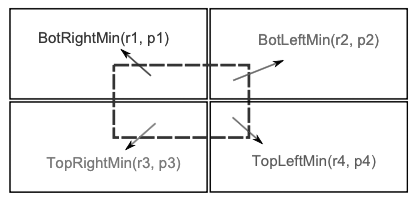
\includegraphics[height=3cm,]{img/yuan2d.png} }
%    \caption{4 \emph{DominanceMin} structure for querying 2D \emph{RMQ}}%
%    \label{fig:yuan2d}%
%\end{figure}

\section{2D RMQ: Querying}
\begin{center}
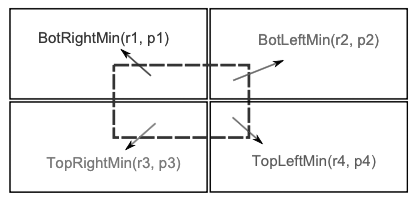
\includegraphics[height=3cm,]{img/yuan2d.png}

\end{center}

For any query range $q$, we can always divide it into 4 parts or canonical ranges, which are all pre-computed and each subquery is a 2-side range query with some canonical range. The above figure shows how the query is splitted into 4 canonical ranges \emph{BotRightMin}, \emph{BotLeftMin},\emph{TopLeftMin},\emph{TopRightMin} respectively.
Hence the final result can be obtained with at most 3 comparisons. However to find this canonical ranges in constant time, Yuan et al. defines the faster approach same as 1D where auxiliary tree for $CIS_1$ and $CIS_2$ are built in linear space and time. \\
\begin{theorem}[Querying Complexity]
With the linear-comparison preprocessing for a 2D array, it takes at most 3 comparisons to answer a range minimum query.
\end{theorem}
%\newpage
\section{RMQ in Higher Dimensions ($d > 2$)}

\section{Preprocessing Stage}
\compress
\begin{itemize}\topsep0pt \itemsep1pt \parskip0pt \parsep0pt
\item Build the canonical interval set for each dimension $1 \leq k \leq d$. Let's call it $CIS_k$ for the $k^{th}$ dimension $[1..n_k]$. Let's denote the set of canonical ranges by $CR = \prod\limits_{k=1}^d CIS_k$.
\item Now within each range $r$ precompute the following data structure for $x \in r$. \[DominanceMin(r,{\bf u},{\bf x}] = \min_{i \in r \cap Dom({\bf x}, {\bf u})} A[i] \]
Now this is the generalization of $2D$ case, here ${\bf u} \in \{-1,1\}^d$ signifies direction. ${\bf i}$ is a $d$-length vector and $Dom({\bf x}, {\bf u})$ is a vector ${\bf p}$ that satisfies $u_k(p_k-x_k) \geq 0$ where $1\leq k\leq d$.
\end{itemize}
\section{Speeding up DominanceMin Structure computation}
Similar to $2D$ case, dynamic programming is used to speed up the computation with the following considerations
\compress
\begin{itemize}\topsep0pt \itemsep1pt \parskip0pt \parsep0pt
\item Sort the canonical ranges
\item During bottom-up merging choose the longest-length dimension ($l=\max_{1\leq k\leq d}\left\vert I_k\right\vert$) for the binary search.
\end{itemize}
The number of comparisons for a range $r=I_1\times I_2\times\ldots xI_d$ becomes $2^d\left\vert r\right\vert\frac{\log l}{l}$.
\section{Query Stage}
As for $2D$ a query could be decomposed to $4$ subqueries, here it can be decomposed to $2^d$ subqueries. The subquery can be answered directly from $DominanceMin$ structures that are precomputed. A subquery can be identified by $d$ nearest common ancestor queries.

\begin{theorem}[Preprocessing Complexity]
The algorithm preprocesses a $d$-dimensional array in at most $B(d)N$ comparisons, where $B(d)=\mathcal{O}((2.89)d\cdot(d+1)!)$
\end{theorem}
\emph{Proof:} Let $R(l)$ and $R'(l)$ be $CR$s with the longest dimension at \emph{most} and \emph{exactly} $l=2^j$ for some $j$ respectively. Then we have the following
\begin{align}
\label{rl}
R'(l)=R(l)\setminus R(l/2)
\end{align}\par
Let $P'_0(l)$ and $P'(l)$ be the total no of comparisons for building $DominanceMin$ structure of $R'(l)$ using naive ($2^d\left\vert r\right\vert$) and binary search ($2^d\left\vert r\right\vert\frac{\log l}{l}$) approach respectively. Similarly let $P_0(l)$ and $P(l)$ be the total no of comparisons for building $DominanceMin$ structure of $R(l)$ using naive and efficient merging algorithm. Because there are $\prod_{1\leq k\leq d}\frac{n_k}{2^{j_k}}$ $CR$s of size $2^{j_1}\times 2^{j_2}\ldots \times 2^{j_d}$ and each brute-force merging costs $2^d\prod_{1\leq k\leq d}2^{j_k}$ comparisons the following can be derived
\begin{align}
\label{pl}
P_0(l)&=2^d\prod\limits_{1\leq k\leq d}\;\sum\limits_{0\leq j\leq \log l}\frac{n_k}{2^j}\cdot2^j=2^d\prod\limits_{1\leq k\leq d}((1+\log l)\cdot n_k)=2^d(1+\log l)^dN\\
\label{p'l}
P'_0(l)&=P_0(l)-P_0(l/2) \leq P_0(l) \hspace{233pt}\text { from equation \eqref{rl}}\\
\label{lgl}
P'(l)&=\frac{\log l}{l}P'_0(l) \hspace{160pt}\text { $\frac{\log l}{l}$ factor improvement due to binary search}
\end{align}\par
Let total no of comparisons for all $CR$s using efficient merging be $P=P(\max_{1\leq k\leq d}n_k)$. So $P=\sum_{i\geq 0}P'(2^i)$. Now using Eqn.\eqref{lgl}, Ineq.\eqref{p'l} and Eqn.\eqref{pl} it can be derived that $P=\sum_{i\geq 0}2^d\frac{i}{2^i}(1+i)^dN$. Therefore,
\begin{align}
\label{bd}
B(d)\leq \frac{P}{N} \leq 2^{d+2}\sum\limits_{i\geq 0}\frac{i^{d+1}}{2^{i+1}}
\end{align}
Now as $\sum_{i\geq 0}\frac{i^{d+1}}{2^{i+1}}$ is finite, this is an ordered Bell number $b(d+1)$\cite{p18}. Using the known complexity of Bell numbers, we get
\begin{align}
\label{bd}
B(d)=2^{d+2}b(d+1)=2^{d+2}\mathcal{O}((1.443)^{d+1}(d+1)!) = \mathcal{O}((2.89)^d(d+1)!)
\end{align}
%\newpage
\begin{theorem}[Query Complexity]
The number of comparisons to answer a $d$-dimensional query is $2^d-1$.
\end{theorem}
\emph{Proof:} With the preprocessed data structure any online query can be divided into $2^d$ subqueries each of which can be answered directly from $DominanceMin$ structure of some $CR$ without any comparison. And $d$ Nearest Common Ancestor query is enough to find out $2^d$ $CR$s. Therefore $2^d-1$ comparison is sufficient to answer any Range Minimum Query.
\section{Implementation in RAM Model}
\section{Micro Data Structure}
The key idea is to divide the input array into micro-blocks with the following properties. 
\compress
\begin{itemize}\topsep0pt \itemsep1pt \parskip0pt \parsep0pt
\item Each dimension of $d$-dimensional microcube is $g=(\epsilon\log N)^{1/d}$, size $G=\epsilon\log N$.
\item Type of a microblock is a sequence of comparison results ($0/1$) from the linear-time preprocessing algorithm. Micro-blocks with same type share same data structure.
\item It takes $B(d)\epsilon\log N$ comparison to preprocess a block and it is so chosen that $\epsilon < \frac{1}{B(d)}$, therefore total no of distinct micro-block types is $2^{B(d)\epsilon\log N} = N^{B(d)\epsilon} = N^f$ where $f < 1$, implies \emph{sublinear}.
\item Types can be recognized using linear-depth ($B(d)G$) decision tree according to the preprocessing algorithm.
\end{itemize}
\section{Decision Tree: Indices Structure ($1D$)}
The key idea here is to store indices of the minimum element for each type of microblock for all possible queries instead of the actual element. This greatly reduces both the space and time complexity of the algorithm, as the number of distinct micro-block type is sublinear. Let's say $PosLeftMin(I,x)$ and $PosRightMin(I,x)$ calculates indices of $LeftMin$ and $RightMin$. Now a structure called $Indices(t,q)$ stores these candidates for each query and $Indices(t,q)[i]$ where $0\leq i\leq1$ is the index of $i^{th}$ such candidate for query $q$ in type $t$ micro-block. The tree has the following properties
\compress
\begin{itemize}\topsep0pt \itemsep1pt \parskip0pt \parsep0pt
\item It is similar to a deterministic program that accepts size of input array and is allowed to call a compare function but can not access elements in the input directly
\item Each internal tree node holds a program state, i.e. a comparison function with indices for the array entries to compare.
\item Root stores $PosLeftMin(I(x),x) = x$,$PosRightMin(I(x),x) = x$ $\forall$ $1\leq x\leq g$ and canonical interval $[x,x]$.
\item Each leaf of the decision tree contains a configuration representing the halting state of the program, that is the Indices structure.
\item Two children of each node represent results of comparison
\item Path from root to any leaf corresponds to a micro-block type
\end{itemize}
\begin{lemma}
The total time and space (in terms of bits) complexities for constructing the micro data structures are $\mathcal{O}(B(d)N)$.
\end{lemma}
\emph{Proof:} Total no. of decision tree nodes is $\mathcal{O}(2^{B(d)G})$, each node costs $\mathcal{O}(G\log^dG)$ time and $\mathcal{O}(G\log^{d+1}G)$ bits space, therefore total complexity is $\mathcal{O}(2^{B(d)G}\cdot G\log^{d+1}G)$. $Indices$ structure costs a total $\mathcal{O}(2^{B(d)G}\cdot G^2)$ time and $\mathcal{O}(2^{B(d)G}\cdot G^2\log G)$ bits. Each microcube type can recognized by walking down the entire depth of the tree therefore $\mathcal{O}(B(d)G)$ and can also be stored using $\mathcal{O}(B(d)G)$ bits. Now $B(d)G<B(d)\epsilon\log N<\log N$, so total space for $\frac{N}{G}$ microcubes is $\mathcal{O}(N/G\cdot B(d)G)=\mathcal{O}(B(d)N)$. Therefore, total complexity of building micro-data structure is $B(d)N+2^{B(d)G}G^2 \leq B(d)N+2^{B(d)\epsilon\log N}(\epsilon\log N)^2 = \mathcal{O}(B(d)N)$.

\section{2D Micro-block Example}
\begin{center}
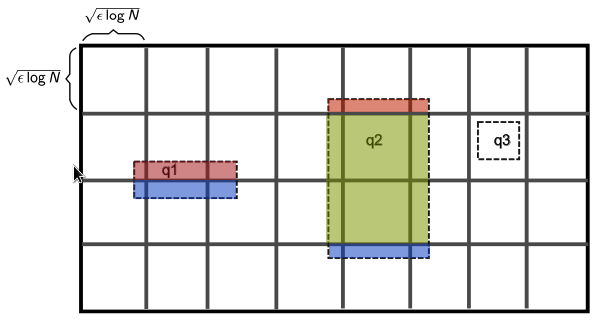
\includegraphics[height=4.5cm,]{img/2dmicro.png}
\end{center}


%\newpage
\section{Query that fits completely in a microcube}
Consider the example in the above picture for query $q3$, it is contained inside one microblock. Therefore, first the microblock type would be looked up from the decision tree, and then $4$ candidates indexed by $Index(t,q)$ would need to be compared to get the minimum. In a $d$-dimensional scenario, there can be upto $2^d$ candidates for comparison.
\section{Query that crosses boundary of one or more microcubes}
Let's consider the queries $q1$, $q2$. $q1$ crosses $1$ micro-block boundary in horizontal direction and $2$ boundaries in vertical direction. And $q2$ crosses $3$ boundaries in horizontal direction and $2$ in vertical direction. 
Now the process of answering such a query in the general case can be described as the following,
\compress
\begin{itemize}\topsep0pt \itemsep1pt \parskip0pt \parsep0pt
\item Choose any one dimension where the crossing occurs. Without loss of generality consider that it is the $1^{st}$ dimension ($n_1$), Let's call the intervals $I_j=[g(j-1)+1,gj]$ where $1\leq j\leq n_1/g$. Now assume the query is $q=[x_1,x_2]\times q'$ where $q'$ is $(d-1)$-dimensional range. For the two examples let's choose dimension $1$ (horizontal). i.e. along $y$ axis.
\item Now assume $[x_1,x_2]$ spans over the intervals $I_u,I_{u+1},\ldots,I_v$, therefore we can divide the query into three parts $q_1=(I_u\cap[x_1,x_2])\times q'$, $q_2=(I_v\cap[x_1,x_2])\times q'$ and $q_3=(\cup_{u<w<v}I_w)\times q'$ where $u=\ceil*{\frac{x_1}{g}}$ and $v=\ceil*{\frac{x_2}{g}}$. And the query $q$ can be answered by taking union of these three. In the example, for $q1$ $u=2,v=3$ and for $q2$ $u=1,v=4$.
\item The following $(d-1)$-dimensional array needs to be precomputed by aggregation.
\begin{align}
\label{a'}
A'_{k,x}(i_1,\ldots ,i_k,i_{k+1},\ldots, i_d)=\min_{x\leq i_k	\leq g\ceil*{\frac{x}{g}}} A(i_1,\ldots,i_d) \text{ where } 1\leq k\leq d, x\in [1,n_k]
\end{align}
This simply computes and stores the results of every $(d-1)$-dimensional subarray where the range of indices of the fixed dimension ($k$) are all suffix of a corresponding micro-block ($\ceil*{\frac{x}{g}}$) along that dimension. This in someway is kind of similar to $RightMin$ for the case of $1D$. Now a query like $q_1$ can be answered from the above because $\min A[q_1]=A'_{1,x_1}[q']$. This would give us the min for red regions in query $q1$ and $q2$.
\item Similarly the following structure needs to be precomputed which can answer a query like $q_2$
\begin{align}
\label{a''}
A''_{k,x}(i_1,\ldots ,i_k,i_{k+1},\ldots, i_d)=\min_{g(\ceil*{\frac{x}{g}}-1)+1\leq i_k	\leq x} A(i_1,\ldots,i_d) \text{ where } 1\leq k\leq d, x\in [1,n_k]
\end{align}
This simply computes and stores the results of every $(d-1)$-dimensional subarray where the range of indices of the fixed dimension ($k$) are all prefix of a corresponding micro-block ($\ceil*{\frac{x}{g}}-1$) along that dimension. This in someway is kind of similar to $LeftMin$ for the case of $1D$. This would give us the min for blue regions in query $q1$ and $q2$.
\item The $(d-1)$-dimensional structures in \eqref{a'} and \eqref{a''} needs to be recursively preprocessed
\item To efficiently answer a query like $q_3$ which covers one or multiple full-sized intervals across some dimension one needs to pre-aggregate the array $A^*_1=\frac{n_1}{g}\times n_2\times\ldots\times n_d$ and preprcoss it using a technique mentioned in next lemma \ref{dim}. The pre-aggregation in general can be done like the following.
\[A^*_k(i_1,\dots,i_{k-1},i^*_k,i_{k+1},\ldots i_d)=\min_{g(i^*_k-1)+1\leq i_k\leq gi^*_k}A(i_1,i_2,\dots,i_d) \text{ for } 1\leq k\leq d\]
This is a \emph{\bf Macro Data Structure} that computes and stores aggregatead result of subarrays spanning over multiple micro-blocks (exact boundaries) along a particular dimension. Now answering $q_3$ on $A$ is equivalent to answer $[x^*_1,x^*_2]\times q'$ on $A^*_1$ where $x^*_1=\ceil*{\frac{x_1}{g}}$ and $x^*_2=\ceil*{\frac{x_2}{g}}$. In the above example the green region of $q2$ can be answered by this. The query $q1$ do not have such a part therefore only $q_1$ and $q_2$ is enough to answer $q1$.
\end{itemize}
\begin{lemma}
\label{dim}
For any fixed d, there is an algorithm to preprocess a $d$-dimensional array using $\mathcal{O}(N(3\log\log N)d)$ time and space (in words), and answer the range minimum query in $\mathcal{O}(3^d)$ time.
\end{lemma}
\emph{Proof:} The min operator fits is in semigroup model. For the 1-dimensional case, Yao \cite{p17} presented an algorithm to preprocess an array using $\mathcal{O}(n\log\log n)$ time and $\mathcal{O}(n\log\log n)$ space (in terms of semigroup elements) to support range sum query, where the query is answered by summing $3$ semigroup elements. Using this as a base scheme in the dimension reduction algorithm of Chazelle and Rosenberg\cite{p3}, we get an $\mathcal{O}(N(3\log\log N)d)$ time and space preprocessing algorithm to support $\mathcal{O}(3^d)$-time range semigroup sum query. Their algorithms can be implemented in the RAM model without changing the complexities.
%\newpage
\begin{theorem}
For any fixed $d$, there is an algorithm to preprocess a $d$-dimensional array using $\mathcal{O}(B(d)N)$ time and $\mathcal{O}(2^dd!N)$ additional space (in words), and answer the range minimum query in $\mathcal{O}(3^d)$ time.
\end{theorem}
\emph{Proof:} Let $T(N,d)$ be total time  required for preprocessing the input array. Then we have
\begin{align}
T(N,d)&\leq \sum\limits_{1\leq k\leq d}\big(2n_kT(\frac{N}{n_k},d-1)+\mathcal{O}(N))+\mathcal{O}(B(d)N)\nonumber & T(N,1)=\mathcal{O}(N)\nonumber &\text{ where } \prod\limits_{k=1}^dn_k = N
\end{align}
Let $S(N,d)$ be total extra space required for the preprocessing. Now $W$ being word size we have
\begin{align}
S(N,d)&\leq \sum\limits_{1\leq k\leq d}\big((2n_kS(\frac{N}{n_k},d-1)+\mathcal{O}(N))+\mathcal{O}(\frac{B(d)N}{W})\nonumber & S(N,1)= \mathcal{O}(N)\nonumber &\text{ where } \prod\limits_{k=1}^dn_k = N
\end{align}
And $Q(d)$ be the query time. So we have
\begin{align}
Q(d)&\leq 2Q(d-1) + \mathcal{O}(3^d) & Q(1)=\mathcal{O}(1)\nonumber
\end{align}
Using Eqn. \eqref{bd} and recursion tree technique we can solve the three recurrences to get
\begin{align}
T(N,d)&=\mathcal{O}(B(d)N) & S(N,d)&=\mathcal{O}(2^dd!N) & Q(d)&=\mathcal{O}(3^d)\nonumber
\end{align}

\section{Conclusion}
\subsection*{Impact of the Results}
The range minimum query problem has direct impact in several fields related to string pattern matching, text compression, genomic sequence analysis in computational biology and image  processing. It also has applications in OLAP databases where multidimensional range min/max queries are used extensively.\par
Recently Brodal et al.\cite{p11} proposed a space efficient indexing data structure for two-dimensional RMQ problems that improves upon the $O(NlogN)$ bits or $O(N)$ words data structure proposed in this paper. Their paper uses the concept of Fibonacci lattice that has applications in the field of graphics and image processing. The paper by Mitzi et al.\cite{p12} explores the problem of expensive updating of prefix sum cubes for OLAP range queries on flash memory. This is based upon the theoretical research work being done on developing efficient data structures and algorithms that focus on range query computations for a given set of dimensions. Farzan et al. \cite{p14} presented a fully compressed representation of a set of m points on an $n \times n$ grid that uses encoding in higher dimensions. This is again inspired by Yuan's contribution.
\subsection*{Future Work}
Although this paper has shown remarkable improvements from the previous techniques used, still it leaves some scope of improvements which we would like to have in the future. 
\compress
\begin{enumerate}\topsep0pt \itemsep1pt \parskip0pt \parsep0pt
\item From this paper we obtain an upper bound on the linear comparisons required at the preprocessing stage. However this leaves open one question that if $t$ comparisons are allowed at the querying stage then what can be the minimum number of comparisons at the preprocessing stage. A major improvement would be to obtain a tradeoff between the number of comparisons at the querying and preprocessing stage. Demaine et al. has shown some results for Cartesian trees, but an improvement would be extend the results for canonical trees.
\item \textbf{Dynamic Updates: }The array considered for range min queries in this paper, are assumed to be fixed. Any update to any position of the array would invalidate the entire preprocessing data structure. Hence it is again required to preprocess the entire data structure before querying stage. The data structure suggested by Poon \cite{p6}
will be much less impacted by such dynamic updates. Hence in the future, a major improvement would be to have space efficient data structures and algorithms which would enable dynamic updates on canonical trees.
\item This paper has based its solution for range minimum query problem on the RAM model. However we still do not know its impact in the external memory model environment. What remains to be seen is that what will be the cost of implementing macro/mircro data structures and the number of comparisons required for the querying and preprocessing stages.
\end{enumerate}
\par

\newpage
\bibliographystyle{plain}
\bibliography{references}

\end{document}